\subsection{Brugeroprettelse}
\label{subsec:brug-opret}

Alle har mulighed for at oprette en bruger på \Foodl{}. Hvis man har en bruger og logger ind på systemet, så kan man kan gemme sin indkøbsliste og listen over favoritter. Det er dog ikke obligatorisk at have en brger for at kunne bruge systemet, da vi ikke ønsker at binde brugerne til at oprette noget som helst. Man kan bruge systemet, om man har en bruger eller ej. 

Man opretter en bruger på samme side, hvor man logger ind på systemet. Dette er præsenteret i \figref{fig:overblik-brugeroprettelse}. Man navigerer til denne side ved at klikke på ``log ind / opret bruger'' i højre side af sidehovedet, som også er synlig på samme figur.

\begin{figure}[H]
	\centering
	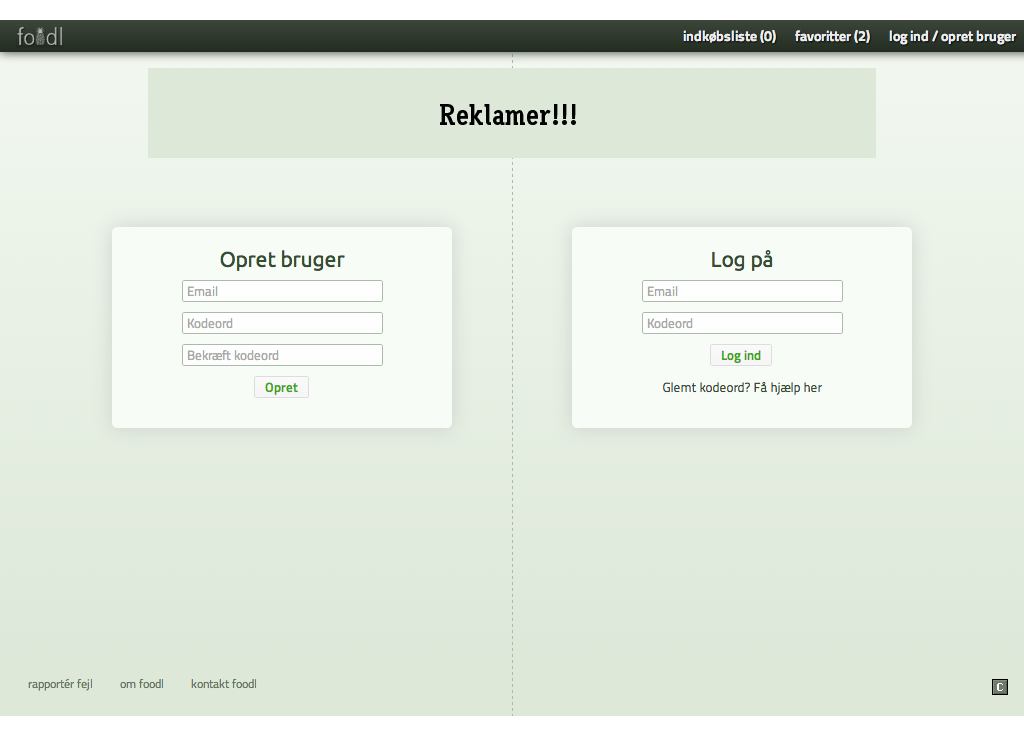
\includegraphics[scale=1]{billeder/foodl/thumbnails/opretbrugeroglogind.png}
	\capt{Denne figur har til formål at give et overblik over systemets brugeroprettelsesside.}
	\label{fig:overblik-brugeroprettelse}
\end{figure}


%\begin{figure}[H]
%	\centering
%	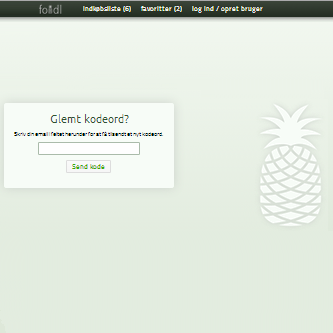
\includegraphics[scale=1]{billeder/foodl/thumbnails/glemtkode.png}
%	\capt{Denne figur har til formål at give et overblik over systemets side, hvor brugere har mulighed for at få tilsendt glemte kodeord.}
%	\label{fig:overblik-glemtkode}
%\end{figure}

%\begin{figure}[H]
%	\centering
%	
\includegraphics[scale=0.7]{billeder/foodl/header.jpg}
%	\capt{Denne figur viser webapplikationens sidehoved, hvilket kan ses på alle undersider.}
%	\label{fig:foodl-header}
%\end{figure}

Man skal bruge sin email og en adgangskode for at lave en bruger. Hvis man allerede har en bruger, så skal man blot logge ind med de rigtige oplysninger.

Når man er logget ind, så ændrer sidehovedet sig en smule. Figur \ref{fig:foodl-loggetind} viser, at der nu er mulighed for at gå ind i en menu, der hedder ``indstillinger'' og at logge ud igen. Man kan også se, at der pludselig er indlæst en liste af favoritter på 10 opskrifter fra tidligere besøg.

%\begin{figure}[H]
%	\centering
%	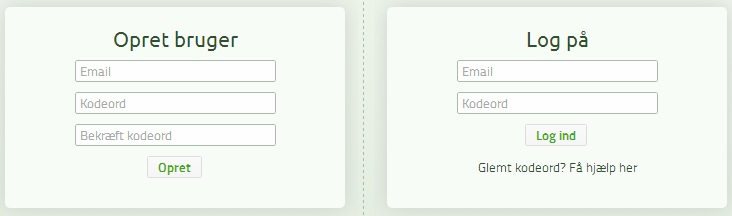
\includegraphics[scale=0.7]{billeder/foodl/login-opret.jpg}
%	\capt{Webapplikationen giver brugeren mulighed for at oprette en bruger og logge ind med denne.}
%	\label{fig:foodl-opret}
%\end{figure}

\begin{figure}[H]
	\centering
	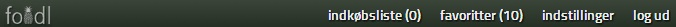
\includegraphics[scale=0.7]{billeder/foodl/header-login.jpg}
	\capt{Det ændrede sidehovede, når brugeren er logget ind.}
	\label{fig:foodl-loggetind}
\end{figure}

Hvis man ønsker at skifte sin adgangskode, så sker det ved at trykke på knappen ``indstillinger'' i sidehovedet.

%\begin{figure}[H]
%	\centering
%	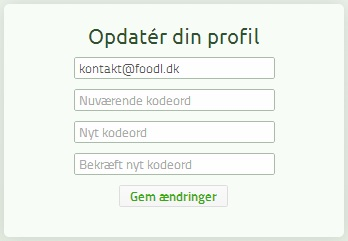
\includegraphics[scale=0.7]{billeder/foodl/indstillinger.jpg}
%	\capt{Brugeren har mulighed for at ændre nogle basale indstillinger ved at klikke på ``indstillinger'' i sidehovedet.}
%	\label{fig:foodl-indstillinger}
%\end{figure}